\chapter{Introduction}

\subsection{Scope}
% TODO: write
\subsection{Publications}
% TODO: write
\subsection{Collaborators}
% TODO: write

\section{Individual cells as complex machinery}
Cells are the basic building block of life -- all living organisms are composed of one or more cells.
They can be considered as complex machines engineered over billions of years of evolution,
which have resulted in intricate cellular "programs" that determine the identify, behavior, and interactions of cells with each other and their environments.
These programs perform a wide range of functions necessary for life, including metabolism, growth, reproduction, response to stimuli, and adaptation to environment.

Recent technological advances in single-cell biology have revolutionized the way scientists are able to study cells.
The development of \emph{single-cell profiling technologies} enable measurements at the resolution of individual cells,
promising a better understanding of cellular development and interaction, with particular implications in the study of cancer.
This data is quite difficult to analyze, as reflected by the underlying complexity of cellular biology, and
computational tools have proven to play an important role in unlocking the full potential of these technologies.
This thesis is largely concerned with the development as well as application of such machine-learning based computational tools to problems tackled with single-cell profiling technologies.

The goal of this chapter is to give a high level introduction to the basics of cellular biology in order to properly motivate the context and intracies of the single-cell data within this thesis.
The hope here is that it useful for readers with a non-biological background, such as those coming from a machine learning field that who would like to gain a better understanding of the powers underneath their data.

\subsection{central dogma}
At the core of each cell's identity is the \emph{genetic code}, a long sequence encoded biologcally as DNA molecules.
This code acts as a "blueprint" for cellular processes and
is replicated and propogated as part of the cellular life cycle.
While the genetic information of cells within an individual human (or another complex multi-cellular organism) is essentially conserved, their cells take on a myriad of different forms and functions.
For instance, different \emph{cell types} -- skin cells, red blood cells, liver cells, nerve cells, etc -- within an individual all share the same genetic information despite exhibiting vastly different appearances and roles.
Thus, not just the content of the genetic code, but how the genetic code is processed plays a critical role in determining the cell.

The \emph{central dogma} is a paradigm that describes this process of extracting genetic information.
Cellular behavior is driven in large part by protein molecules which exert influence through chemical interactions within their inter- and intra-cellular environments.
In essence, proteins are one-dimensional sequences of twenty distinct organic compounds known as amino acids and are constructed from interpretation of the genetic code.
On a high level, genes, particular sections of the genetic code stored in the form DNA, are transcribed into a corresponding RNA molecule, which are then translated into some specific protein.
While the reality is more complicated, the information flow generally flows from DNA to RNA to proteins.

An overview of the essential characteristics of each level in the central dogma is given below:

\paragraph{DNA} The genetic code is stored in the form of DNA (dioxyribose nucelic acid) molecules.
These long polymer chains are sequences of only four unique monomers called nucleotides.
When a cell divides, its DNA is replicated such that the daughter cells are composed of identical copies of the genetic code.
As DNA forms the base of the central dogma, the root of the information flow, it is important that its makeup is conserved.
While DNA famously exhibits a double-stranded helical structure,
each nucleotide has a unique corresponding partner whose bonds connect the two strands.
The genetic code, as represented by DNA, is often regarded as a one-dimensional string.
This double-stranded structure represents a redundancy in information and is exploited by cellular processes aimed at conserving the integrity of the genetic code.
Furthermore, in eukaryotic cells, from which all multi-cellular organisms (fungi, plants, and animals) are comprised, DNA is stored within the nucleus of the cell.
The nucleus protects the DNA with its own membrane that regulates the flow of chemical entities in and out of it and the DNA itself generally does not leave the nucleus \cite{milo2015}.

\paragraph{RNA} RNA (ribonucleic acid) is the intermediate step in the central dogma and plays a central in gene expression and regulation.
Since DNA is typically secured and isolated from interacting with the cellular environment, RNA can be understood as its intermediary.
RNA is constructed in a process called \emph{transcription}, where DNA is unwound and converted into RNA.
Like DNA, RNA is composed of a sequence of four unique nucleotides, which are the same as DNA except that thymine (T) is replaced with uracil (U).
In a processes called \emph{translation}, RNA strands are read to create specific proteins.
In this way, RNA plays the central role in gene expression, determining what proteins are created as well as the rate of their creation.
As the cells of a single organism share the vast majority of their DNA, 
gene expression is what allows them to differentiate and specialize.
Gene expression is also used to understand what processes the cell activates or de-activates due to changes in its environment.

\paragraph{Proteins} Proteins represent the ultimate stage of the central dogma and are largely responsible for the behavior and general function of a cell.
Like DNA and RNA, proteins can be conceptualized as one-dimensional sequences over an alphabet of twenty \emph{amino acids}.
During translation, this amino acid sequence is read from the genetic code where triplets of RNA nucleotides are converted into a single amino acid.
Proteins, however, have complicated 3D shapes that are fundamentally tied to its functions.
In a process known as \emph{protein folding}, chemical interactions between a protein's amino acids cause it to contort, yielding these complicated 3D structures.
Hemoglobin, for instance, a protein found in red blood cells that plays a critical role in the transport of oxygen, has a 3D shape that interacts chemically with oxygen molecules in order to absorb and release them.

\subsection{Pathways and cellular signaling}
Cellular processes are controlled and executed, in large part, via signals to proteins encoded as chemical interactions
While the 3D form of a protein largely determines its function,
these forms are not static and can change,
either through the breaking and reforming of bonds between a protein's amino acids,
or through the binding of some external chemical object.
Returning to the example of oxygen transport by hemoglobin -- the function of hemoglobin is to i) bind oxygen in the lung and ii) release it throughout the body.
Hemoglobin has two stable conformations that favor either the capture or release of oxygen molecules.
The preferred conformation is driven by chemical interactions determined by pH and oxygen concentration of the environment \cite{riggs1971}.

A common form of cellular signaling occurs when a protein and some external chemical object interact through the formation of chemical bonds.
An entity that binds to a protein is called a ligand and these ligands can range in complexity from simple ions to entire proteins.
Protein-ligand interactions are complex and are typically made with multiple bonds across many amino acids within the protein, often in the form of some "pocket" or "cavity" within the protein's 3D shape.
Resulting from this complexity, proteins have a high specificity for ligand binding and are usually only able to interact with few ligands.
Ligand binding can, for instance, change or stabilize a protein's shape, influence its chemical properties, form multi-protein complexes, etc, thus changing its shape and therefore function.

Major cellular processes, interactions, and responses are governed through complex and highly regulated signaling hierarchies called \emph{pathways}.
These pathways are composed of, typically, dozens of proteins that illicit cellular response through the capturing and relaying of chemical signals from the external cellular environment into the cellular interior.
Signaling within these pathways is often carried out through ligand binding that can \emph{activate} or \emph{deactivate} proteins, i.e. change their properties such that they included or excluded from participating in some cellular action.
Pathways govern fundamental cellular decisions, for instance, dictating how and when to grow, divide, differentiate, die, etc.
These decisions are typically enacted through the activation (or deactivation) of some key protein, or by ordering the transcription and translation of some specific gene.
Figure \ref{fig:hallmarks} depicts the general structure of a signaling pathway and a cartoon of the MAPK-ERK pathway, a pathway essential to regulating cell growth.

% TODO: adapt figure better
\begin{figure}
  \begin{center}
  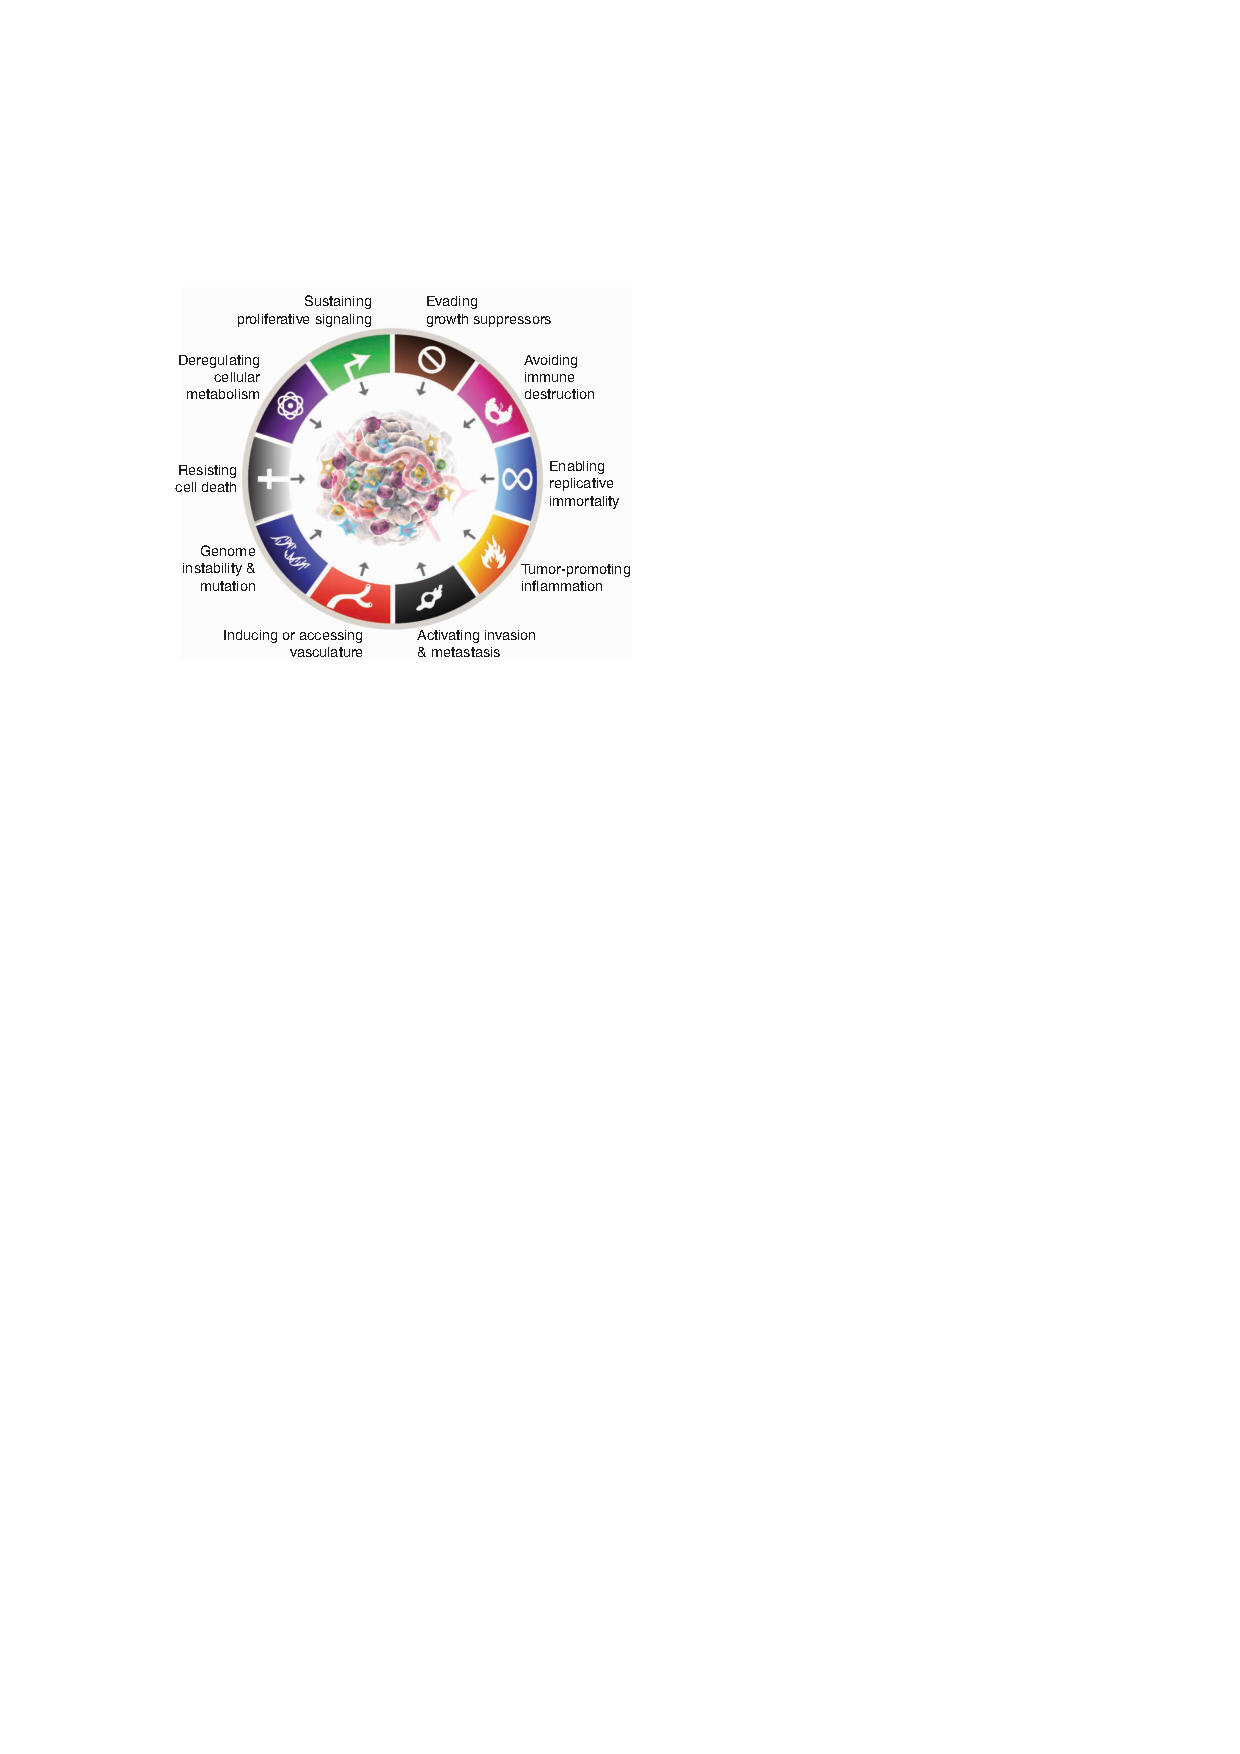
\includegraphics[width=0.95\textwidth]{figures/introduction/hallmarks.pdf}
  \end{center}
  \caption{Hallmarks of cancer, adapted from \cite{hanahan2011}}
  \label{fig:hallmarks}
\end{figure}


\paragraph{Centralized pathway databases}
Centralized databases of cellular signaling pathways are important resources to the biological research community.
These databases are curated through a combination of manual curation, literature reviews, and computational approaches, and distill the last few decades of cell biology research.
Reactome \cite{vastrik2007} and the Molecular Signatures Database (MSigDB) \cite{liberali2014} are two prominent centralized databases of cellular signaling pathways.
Reactome is a curated database of human biological pathways, including metabolic, signaling, and disease pathways.
It provides a comprehensive view of cellular processes and their interconnections.
MSigDB is a collection of gene sets expertly curated and automatically generated that represent a wide range of biological processes and signaling pathways.
Their "Hallmark" gene set contains a refined set of 50 pathways that represent essential gene functions.
These databases are widely used for pathway analysis, gene set enrichment analysis, and network analysis to understand cellular responses to different stimuli.
Other prominent databases in this field include KEGG \cite{kanehisa2000}, Biocarta \cite{nishimura2001}, and WikiPathways \cite{agrawal2024}.
These resources are crucial for understanding cellular signaling and identifying key regulators of biological processes.

\subsection{Genotype, phenotype, and mutations}
A useful abstraction is the distinction between an organisms's \emph{genotype}, the full set of information contained in its genetic code, and its \emph{phenotype}, its observable characteristics.
As we have seen, this relationship is far from one-to-one -- there are many factors beyond the genetic sequence that regulate and influence processes like transcription and translation.
However, it can happen that \emph{mutations}, changes in the genetic sequence, produce drastic effects on the phenotype.
For example, while redundancies exist between the 64 unique nucleotide triplets and the 20 unique amino acids they code for, changes to genetic code can sometimes cause a different amino acid to be translated.
If this change occurs within some important location within the protein, such as one critical to its shape or structure of a ligand binding site, the intended function of the protein can be invalidated.
Returning again to hemoglobin, the genetic disorder sickle-cell anemia is caused by a point mutation, a single nucleotide change in the genetic code, that alters the shape of the protein such that it cannot bind oxygen, to devastating effect.
As we will see, mutations play a critical role in the development of cancer, albeit in more nuanced and/or complicated contexts.

\section{Hallmarks of Cancer}
Cancer is a family of genetic diseases in which normal cells exhibit abnormal behavior that causes them to grow and proliferate uncontrollably, resulting in a mass of cells known as a tumor.
This growth can lead to serious health complications as cells
can then invade nearby tissues and spread to other parts of the body.
Over the last few decades, the development of effective cancer treatment strategies has been at the forefront of biomedical research and has been the focus of moonshots \cite{thewhitehouse2016} and large international consortia \cite{icgc2020}.
Despite this, cancer has remained an active research environment, challenging researchers to understand and control complex and nuanced cellular behaviors that can often times be specific to the tumor.
Many of the methods developed and applications explored within this thesis are motivated by challenges arising from understanding and treating cancer.

A major complication towards the treatment of cancer lie in the myriad mechanisms cells can use to escape the natural regulatory processes that prevent unchecked growth.
The \emph{Hallmarks of Cancer}, proposed by \citet{hanahan2000} in \citeyear{hanahan2000} and updated in \citeyear{hanahan2011} \cite{hanahan2011} and \citeyear{hanahan2022} \citep{hanahan2022}, is a framework to understand the key capabilities and enabling characteristics of cancer cells.
The framework (Figure \ref{fig:hallmarks}) describes eight capabilities, which can be considered as something akin to "gates" in the sense that they each represent some core regulatory process that must be bypassed in order for a normal cell to become cancerous, a process known as tumorigenesis.
In addition, the framework also describes two enabling characteristics, "Genome instability \& mutation" and "Tumor-promoting inflammation", which describe the general mechanisms used to bypass each "gate" and obtain the property of each hallmark characteristic.
In essence, the framework poses that in order for a cell to become a cancer cell, it must, by way of genetic mutations and tumor-promoting inflammation, both
i) sustain, promote, or generate cell growth signals, and, simultaneously,
ii) ignore or resist growth suppression or death (apoptosis) signals \cite{hanahan2011}.

\subsubsection{Genome instability \& mutations} \label{sec:cancer-mutations}
Genetic mutations are one of the underlying causes that enable cells to gain hallmark capabilities.
These "hallmark-granting" mutations typically change the coding of specific proteins key to cellular regulation.
As a result, these proteins become composed of slightly different amino acids and their shape and therefore function are changed.
This can cause gain or loss-of function, resulting in abnormal activation or deactivation of important cellular pathways.
Mutations in genes coding for these proteins are known as \emph{driver} mutations, as they take some of the core responsibility of guiding or driving tumorigenesis \cite{martinez-jimenez2020}.
identifying and then interrupting or reversing the effects of these driver mutations is a central strategy in cancer treatment.

Mutations in the BRAF gene are one of the most infamous examples of driver mutations.
Cell growth and proliferation are normal aspects of the cell life cycle.
In healthy cells, the signals that govern these processes are well regulated such that normal functions are maintained.
A signature property of cancer cells, on the other hand, is to deregulate these sources, resulting in abnormally high growth signals.
Changes to the BRAF protein, a key member of the RAS/MAPK signaling pathway \cite{davies2011}, a major intracellular signaling cascade that regulates cellular growth and proliferation,
can result in sustained growth-promoting signals.
Around 40\% of human melanomas contain a mutation in the BRAF gene, and 
85\% of these mutations are within the V600E subunit \cite{spathis2019}.
Consequently, many resources have been allocated towards the understanding of this protein, its common mutations \cite{smiech2020}, and treatment strategies \cite{cheng2018}.

Another class of driver mutations occur in so-called "tumor suppressor genes."
These genes code for proteins that are key members of the body's natural regulatory function that detect cancerous abnormalities and, in response, send growth-inhibiting signals \cite{joyce2024}.
Cancer cells must evade or ignore these signals in order to continue to grow unchecked,
typically by interrupting the pathways activated by these signals.
Mutations that interrupt the basic duties of these genes can be particularly harmful.

Mutations can be classified into one of two classes:
\emph{germline} mutations that are inherited and present at birth, or
\emph{somatic} mutations that are acquired throughout one's lifetime, e.g. by smoking, exposure to UV radiation, or simple random chance \cite{hanahan2011}.
A complication towards robust cancer treatments stems from the fact that individuals will have unique mutation combinations and the development of "one-size-fits-all" treatments are difficult or impossible.
Futhermore, while driver mutations appear in some subset of genes, they can affect different subunits and/or have different effects on the proteins downstream behavior \cite{smiech2020}.

As tumor cells proliferate, they copy and propagate their genetic mutations.
Tumor "clones" are genetically (and phenotypically) distinct cancer cells, arising from some original cancer cell.
Cancer cells, when compared to normal cells, are typically more susceptible to acquiring somatic mutations, due to, for instance, mutations in DNA-repair mechanisms \cite{negrini2010,salk2010}.
As a result, the genetics of cancer cells can exhibit a branching process within tumor clones, resulting what are known as tumor subclones.
The presence of these subclones represents a further complication in effective cancer treatment as these are not only specific to the individual but treatments need to address all active subclones which may exhibit differential responses to therapies.

\subsection{"Tumor-promoting inflammation" and the tumor microenvironment}
Inflammation refers to an organism's natural biological response to harmful stimuli,
for instance, the immune system response to a foreign disease.
While it has been known that immune cells interact with and are involved in tumor formation, research over the last few decades has indicated that these interactions are crucial to the behavior of the tumor \cite{grivennikov2010, quail2013}.
This has lead to a sea-change in basic models of cancer -- tumors are not some relatively homogeneous mass of cancer cells experiencing unchecked growth, but a complex orchestra of interacting cells.
Under this tumor microenvironment (TME) model, tumors can be understood as something not unlike an organ that survives and propagates thanks to complex signaling interactions between many different cell types \cite{balkwill2012}, which are, as described above, specific to the individual.
Specifics of the TME have been shown to contribute to immune evasion \cite{pansy2021},
immunospression \cite{balta2021}, and immune cell reprogramming \cite{cao2022}.
It has also been shown that the immune responses within the TME can have 
have the counter-intuitive effect of \emph{promoting} tumor development \cite{hanahan2011}, for instance by supplying factors that promote growth \cite{denardo2010}.

%While the TME is not directly addressed within this thesis it is important to appreciate the underlying sources of tumor heterogeneity that must be captured by methods.
%Emerging spatial transcriptomic technologies \cite{need,need}, capable of measuring, for example, gene expression spatially-resolved at the single-cell level,
%have been shown to be promising directions towards the understanding of the TME \cite{need}.

\subsection{Strategies for treating cancer}
Common strategies to combat cancer usually involve blocking or reversing the specific mechanisms that enable critical hallmark capabilities.
Since the mutations and TME that drive the cancer hallmark capabilities can be unique to the individual,
developing a sweeping, generalized treatment to cancer is difficult.
Instead treatments are typically \emph{personalized} to the distinct mechanisms underlying each tumor.
There are two main approaches to treating cancer:
immunotherapy, which bolster the host immune system to identify and eliminate cancer cells,
and chemotherapy, which target and attack the cancer cells themselves \cite{hanahan2011}.

A class of chemotherapy comes in the form of orally ingested drugs that are designed to interact with specific pathways affected by cancerous mutations.
\emph{Targeted} therapies are a subclass of these chemotherapies that are designed for specific driver mutations.
For instance, the drug dabrafenib targets mechanisms underlying BRAF mutated cancer cells by inhibiting the activity of the BRAF V600E protein \cite{khunger2018}.
In general, these treatments can be conceptualized as perturbations over the heterogeneous makeup of a tumor, in which cells can have differential responses depending on their states, subclones, microenvironment, etc.
Combination therapies are another common strategy where two or more drugs are prescribed that either have synergistic effects or target multiple hallmark capabilities.
This strategy has been shown to be effective across multiple subclones, to bolster a targeted therapy, or to combat aggressive cancers \cite{hanahan2011}.

\section{Single-cell profiling technologies}
%\begin{enumerate}
%  \item even with the simplified view described here, there many information levels that determine cellular behavior
%  \item first advances into studying cell behavior, microscopes, hooke
%  \item nowadays, many technologies exist, taking different profiles of cells, different persepectives, etc
%  \item sequencing vs imaging vs whatever cytof is? 
%\end{enumerate}

Even with the simplified views described here, there are many levels of information -- e.g. DNA, RNA, protein -- that determine and govern cellular behavior.
As consequence, observations made on cells can come in many different forms and flavors that depend on the information or mechanisms of interest.
Omics refers to the some sub-field of cellular biological, typically ending with -omics, that studies some specific level of cellular information.
For instance,
genomics is the study of the complete set of genes in an organism,
transcriptomics is the study of RNA transcripts,
proteomics is the study of proteins,
but also
metabolomics is the study of metabolites,
epigenomics is the study of epigenetic modifications,
and so on.
Nowadays many strategies and technologies have been developed to measure and construct different cellular profiles, at the resolution of individual cells.
Each of these omics require the development of techniques and technologies specific to its profiling.
Within this thesis, methods are developed and applied primarily to transcriptomic and proteomic data.
The relevant technologies and data are described below.

%The measurement of proteomic information has a wider range of approaches, including fluorescent-based imaging and mass spe

\subsection{Transcriptomic profiling with scRNA-seq}
Genetic and transcriptomic information is measured with (single-cell) sequencing technologies that extract fragments of DNA/RNA and identify the sequences of nucleotides 
using so-called sequencing technologies.
These technologies are rooted in the Human Genome project,
a monumental scientific achievement that laid groundwork with the development of "next-gen" sequencing technology.
The human genome contains billions of nucleotides and so measuring this sequence end-to-end is infeasible.
Next gen sequencing technologies instead isolate and measure the nucleotide sequence of small fragments called reads.
The human genome project demonstrated how to assemble a genome, that is piece together the full sequence from overlapping fragments, like a colossal jigsaw puzzle \cite{lander2001}.
While the genome of each individual is distinct, the vast majority is conserved,
so, given some population of individuals, a \emph{reference} genome can be constructed to represent some average or canonical member of the population.
Once a reference is constructed, instead of assembling the code of a new individual from scratch, reads can then be \emph{mapped} onto the reference.

Whereas the human genome project was concerned with the measurement of genomic information,
the measurement of transcriptomic information, i.e. the nucleotide sequences of the free-floating RNA within a cell, follows the same general strategy.
Transcriptomic states are of particular interest as they represent something like a "real-time" snapshot of a cell's current actions.
Bulk sequencing technologies were the first iteration of technologies to measure cellular RNA states.
These technologies pool cells from a heterogeneous multi-cellular sample,
extract the RNA of individual cells, and measure a single signal that represents a composite of RNA states across all cells in the sample.
These technologies offer cheaper but low-resolution profiles, as the information from the individual are grouped together.
Deconvolution methods applied to a population of bulk measurements are popular approaches to infer higher resolution measurements, such as cell-type "signatures".
This approach is still quite limited as they rely on cell states that are conserved across many individuals in the population and we have seen,
such as in the case of cancer, that cellular behavior can be unique to the individual.

The last decade has seen, and continues to see, the development of single-cell sequencing technologies
that have revolutionized our capability to study cellular behaviors and especially in the context of heterogeneity \cite{moty2014}.
These technologies are capable of mechanically isolating individual cells and then sequencing its expressed RNA.
Instead of a single measurement over a sample, single-cell sequencing methods produce observations in the form of large count matrices of cells -x- genes,
where counts refer to the number of reads found in a cell that map to one of its genes.
For reference, humans have on the order of 20k protein coding genes.
While these methods offer deep insight into the inner workings of an individual cell, they must do so at the cost of much less transcriptomic information.
Single-cell technologies rely on a processing step in which successfully captured reads are first replicated before aligned.
The failure rates associated with capturing and replicating reads are thought to cause a "dropout" effect, where the single-cell observation fails to detect genes that are actually expressed.
However, it is understood that, at any given time, cells may express only a small subset of their total genes \cite{adams2008}.
This biological sparsity is then conflated with the technical sparsity due to the dropout effect.
Dealing with the sparsity and (relatively) low information content of this data is a major challenge in the analysis and modeling of single-cell data.
Popular computational strategies utilized in the analysis of scRNA-seq data is explored in section \ref{sec:scrna-seq}.

\subsection{Proteomic technologies}
%\begin{enumerate}
%  \item main challenges in dna/rna stem from extracting and aligning sequencing information
%  \item proteins have macroscopic and checmical properties that can be exploited for profiling
%  \item general strategy: construct some chemical "label" that i) emits an easily identified signal and ii) has a modular group, sometimes called an antibody, that can be engineered to bind to specific proteins of interest
%  \item the single-cell protein abundance is measured, in proxy, by isolating an individual cell and measuring the abundance of the signal emitted by all bound labels
%  \item the main drawback of these methods is their reliance on custom-made antibodies that are specific to a protein of interest
%  \item it requires that the practioneer select what proteins they want to measure apriori to running the experiment
%  \item these proteins are often selected as key proteins within some pathway of interest and are referred to as "markers" as they "mark" for the state of these pathways
%  \item label-free methods attempt to directly measure the chemical properties but come with their own set of computational and signal processing challenges
%  \item here we describe two proteomic profiling technologies that are further explored in this thesis
%\end{enumerate}

Whereas the main challenges in genomic and transcriptomic profiling arise from the extraction and alignment of nucleotide sequences,
approaches for proteomic profiling can exploit the macroscopic and checmical properties of proteins.
As proteins are directly responsible for a large portion cellular identity and behavior, protein profiling in turn offer a "direct" view into the current state of a cell.

There are two main strategies to achieve this profiling.
Label-based approaches target proteins of interest, while label-free approaches attempt to measure all proteins in a cell.
The former approaches are currently more developed than the latter, which comes with their own set of signal-processing challenges.
Label-based approaches require that the proteins of interest are defined apriori and are typically chosen to be key participants in cellular pathways.
These proteins are called "markers" as they "mark" for the activity level of their respective pathway.

The general approach behind label-based proteomic profiling strategies involve constructing some chemical "label" that i) emits an easily identified signal and ii) has a modular group, sometimes called an antibody, that are engineered to bind to unique proteins of interest.
The label abundance within each cell is then measured as a proxy of the cell's protein abundance.
When compared to sequencing, these approaches tend to scale to a larger number of cells, at the cost of measuring fewer biological features.
The number of features a label-based profling methods are limited by the facts that i) the modular groups need to be designed to uniquely bind to specific individual proteins and ii) the signals the labels emit are easy to measure because they have wide "bandwidths" in their obserble spaces
(imagine an old radio that requires clean incoming signals such that such that only a small number of radio towers can effectively communicate with it without overlapping frequencies).
Two such label-based profiling technologies are utilized in this thesis:
CyTOF, which communicates signals in a chemical space, and 4i, which communicates signals in visual space.

\paragraph{CyTOF}
%\begin{enumerate}
%  \item labels are selected for proteins of interest and tagged with heavy metals
%  \item labels bind within their cells, then cells are isolated and atomized
%  \item the chemical composition is then measured using time-of-flight mass spectrometry
%    which stratfies a cloud of ions based on their individual mass-to-charge ratio
%  \item heavy metals are chosen as they have a specific mass-to-charge ratio and do not occurr frequently in biological samples
%  \item protein abundance is then measured by the abundance of the signature ts associated heavy metal emits
%\end{enumerate}
CyTOF (cytometry time of flight) \cite{bandura2009,bendall2011}
measures single-cell protein levels using labels consisting of heavy metals, which tend to appear rarely in biology and have unique signals that are easy to identify.
Once these labels bind to their specific target proteins, cells are first isolated and then atomized, reducing all structures within the cell to their atomic components.
Then atoms are shot through what is essentially a microscopic rail gun and a detector measures how far they travel.
The distance each atom travels is directly related to its mass-to-charge ratio, that is lighter and/or more charged particles are shot farther.
Thus, the atomic cloud is observed in terms of a composite signal over the mass-to-charge ratios of all atoms within.
Protein abundance is then approximated based on the relative abundance of the corresponding levels of detected heavy metal signatures,
which have unique fingerprints in the mass-to-charge space.

\paragraph{4i} % TODO: expand more here
4i (iterative indirect immunofluorescence imaging) \cite{gut2018}
is an imaging-based technology that measures protein levels with immunofluorescent labels.
These labels bind to their target proteins and emit a specific color of light
that is then measured with an extremely high-resoultion camera capable of observing sub-cellular features.
Thus, the protein levels are approximated by the intensity of the colored light emitted by its label.
Furthermore, as the number of available color channels is limited,
4i describes a novel iterative washing and staining protocol that allows for the use of differently labelled color channels.
An image processing pipeline is then used to identify cellular boundaries and extract a set of observables of each individual cell.
These observations include not only the intensity levels of each marker, but morphological features such as cell area, circumference, roundness, etc.

\subsection{Tumor profiler project}
The Tumor Profiler (Tupro) study \cite{irmisch2021} explores the clinical feasibility and utility of applying multi-modal single-cell profiling technologies to precision oncology.
It is a multi-center initiative, of which I am a contributing member, based in Switzerland across the state hospitals, University Hospital Zurich and University Hospital Basel, and academic institutions, ETH Zurich and University of Zurich, with support from the pharmacological industry, including Roche Ltd and NEXUS of ETH.
Its goals (Figure \ref{fig:tupro-overview} are two fold:
1) to demonstrate that a multi-modal single-cell profile of a patient biopsy can be generated and analyzed within a clinically relevant time frame
and 2) that this analysis can inform and improve upon traditional clinical decision making.
Furthermore, in doing so, the project generated a multi-modal single-cell dataset of one of the largest cancer cohorts academically available,
leading to offshoot "exploratory science" efforts.
This project has been a major source of inspiration and data for this thesis.

\begin{figure}
  \begin{center}
    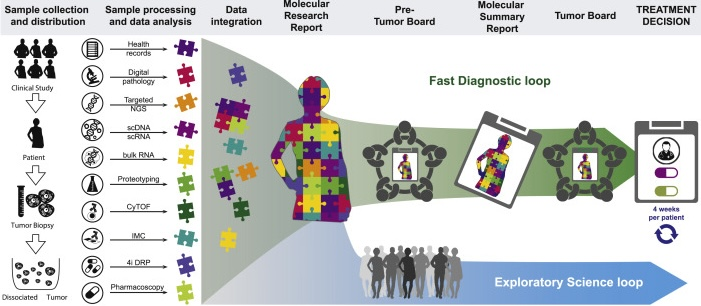
\includegraphics[width=0.95\textwidth]{figures/introduction/tupro.jpg}
  \end{center}
  \caption{}\label{fig:tupro-overview} % TODO: caption, adapted from
\end{figure}

Over the course of three years, the project applied cutting-edge multi-modal profiling technologies to a total of 240 samples spanning metastatic melanoma, metastatic epithelial ovarian cancer, and acute myeloid leukemia.
These samples are derived from biopsies taken from patients enrolled in one of the participating hospitals.
After the biopsy is taken, it is divided and distributed to one of the technology nodes who profile their split with their respective technology.
The single cell profiling technologies described in the previous section are a subset of the total technologies employed by the study.
Analysis from each node is integrated and distilled into a report and 
this report is further distilled by a "pre-tumor" board and finally by the final tumor board where treatment decisions are made.
For each sample, the target turn around time for collection, profiling, and analysis is two weeks.

\section{Representation learning, scRNA-seq} \label{sec:scrna-seq}
Raw read outs of single-cell profiling technologies often have statistical properties that are difficult for computational tools to handle.
These statistical properties, present especially in scRNA-seq but applicable for biological data in general,
include challenges like high-dimensionality, heavy-tailed distributions, sparsity, and noisy observations.
Additionally, there are added challenges due to batch effects, 
technical variations that arise from uncontrollable differences in experimental conditions that can result in differences in the measured gene expression levels between different runs, or batches, of the same experiment.
As such, special care must be paid to not only the normalization of data, but their representation as well.
In this section we detail some of the major sources of noise in scRNA-seq data, how they are addressed or not addressed in common normalization strategies, and autoencoder-based approaches to learn compressed and more manageable cellular representations.

\subsection{normalization, hvg, etc of scRNA-seq}
The usual approach to scRNA-seq involves several steps: read extraction, amplification, and mapping.
Read extraction involves converting RNA molecules into complementary DNA (cDNA) and attaching adapters for sequencing.
Then, amplification via PCR generates millions of copies of the cDNA, which are finally sequenced and mapped to a reference genome.
This ultimately generates a (sparse) cell-x-gene count matrix.
To help alleviate biases arising due to variation during the amplification step, unique molecular identifiers (UMIs), a small nucleotide sequence, are concatenated to captured RNA molecules before amplification \cite{islam2014}.
After amplification, the UMIs remove duplicate reads, reduce the impact of PCR biases, and improve the accuracy of gene expression estimates.

A common challenge in the interpretation and analysis of scRNA-seq data is the disentanglement of biological signal from technical noise.
For instance, the source of the sparsity of expressed genes can arise from both a biological limitation on the number of co-expressed genes a cell is able to exhibit and a technical limitation on the rate of capture \cite{breda2021}.
Thus, preprocessing and normalization of scRNA-seq data rely on intuitions of the underlying biological and technical mechanisms.

There are two main sources of variation underlying the measurements made in scRNA-seq,
variation in the capture reads and variation in the relative rate of replication in the amplification step.
Since RNA molecules are distinct entities, their abundances are modeled using discrete probability distributions.
The Poisson distribution is a popular choice to model these variations,
as the number of RNA molecules or UMIs of a given gene in a single cell is typically conceptualized as a count of independent capture events \cite{breda2021},
which is the key assumption underlying the Poisson distribution.
scRNA-seq data can exhibit additional sources of variations, from both technical sources and dynamics in underlying biological mechanisms \cite{hicks2018},
that break these assumptions.
In such cases, a popular choice is the more complex negative binomial distribution \cite{choudhary2022}.
While many methods have been introduced that utilize the negative binomial distribution \cite{lopez2018, risso2018, eraslan2019},
these methods can, in general, be expensive to fit, be difficult to tune, or rely on statistic models that may or may not be correctly modeling the underlying biology \cite{ahlmann-eltze2023}.

The degree to which sparsity in scRNA-seq data arises from biological or technical origins is a controversial issue.
While missing data or zero gene counts can arise from biologically unexpressed genes, they can also arise from technical artifacts,
such as failure to capture reads before amplification.
So called "zero-inflation" or "gene dropout" refers to genes expressed biologically but reported missing due to these technical effects \cite{silverman2020}.
There was convincing evidence for these effects in the early days of scRNA-seq \cite{vallejos2017},
and likelihood-based models were enhanced with mixture terms to zero out counts \cite{pierson2015, dijk2018, lopez2018, huang2018, eraslan2019}.
Recent arguments, however, challenge the prevalence in current scRNA-seq technologies \cite{svensson2020,jiang2022}
and models with zero-inflation terms have shown to perform similarly when they are removed \cite{vieth2017},
yet these arguments still remain controversial or nuanced \cite{cao2021}

The standard normalization of scRNA-seq data is a two step process involving a simple library size normalization followed by a variance-stabilizing log transform \cite{luecken2019}.
While this normalization does not directly address the variation and mechanisms described above, it has been shown to perform suprisingly well \cite{ahlmann-eltze2023}.
The library size normalization addresses a ubiquitous source of confounding in scRNA-seq data.
Observations are reported in the form of gene counts and the total number of these counts from an individual cell is known as its library size.
The library size is determined due to several underlying technical variations including but not limited to capture rate \cite{lytal2020} and influences the magnitude of gene counts.
Therefore, the library size is typically normalized such that the total number of counts within an individual cell is some constant.
After library size normalization, a variance-stabilizing log transform is applied.
Since many gene counts are still zero, a constant offset or pseudocount is applied, $log(x + 1)$ also referred to as \textit{log1p}, to avoid \textit{nan}s.
There is a relationship between the normalized library size and the pseudocount, as smaller library sizes imply, in effect, larger pseudocounts.
This in turn affects the statistics and behavior of lowly expressed genes \cite{ahlmann-eltze2023}. % TODO: how?

Even after normalization, the sparsity and high-dimensionality of scRNA-seq data still remain as challenges.
In addition to the filtering genes and cells that exhibit a high degree of sparsity, it is commonplace to select for some subset of highly-variable genes (HVGs).
For example, "house keeping" genes, in charge of basic cellular processes, tend to be constantly expressed at high levels and are relatively uninformative to cellular identity.
Furthermore, there may be a large number of genes that mark for specific pathways, cell types, or other biological processes which may not be present or of interest.
HVG selection aims to remove such genes automatically, by determining non-informative genes whose expression does not change across the population.
Oftentimes, this step can reduce the dimensionality from the tens of thousands to the much more manageable hundreds to thousand \cite{satija2015,zheng2017,stuart2019}.

\subsection{autoencoders, vae} \label{sec:autoencoders}
Autoencoders (AEs) have emerged has powerful and ubiquitous tools to aid in the modeling and analysis of scRNA-seq data.
These models learn compressed representations of high-dimensional data by training a pair of neural networks, an encoder $\phi$, and a decoder $\psi$,
to map data into and out of a low-dimensional "bottleneck" feature space such that data points can be faithfully reconstructed from their bottleneck representations.
Let $x \in \mathbb{R}^D$ be a data point in the high-dimensional feature space and let its corresponding representation in the low-dimensional space is $z \in \mathbb{R}^d$.
Then $\phi \mapsto \mathbb{R}^D \to \mathbb{R}^d$ \emph{encodes} data points into the bottleneck feature space,
while the decoder $\psi \mapsto \mathbb{R}^d \to \mathbb{R}^D$ \emph{decodes} data points from the bottleneck feature space back into the data space,
that is $z = \phi(x)$ and $x\prime = \psi(z)$ is the resulting reconstructed data point.
The autoencoder is trained, typically with gradient descent methods \cite{kingma2017} to minimize the reconstruction error:
\begin{equation}
  \mathcal{L}_{ae}(\phi, \psi; x) = -\frac{1}{2} || x - x\prime ||^2
  \label{eq:ae-loss}
\end{equation}

The popular Variational Autoencoders (VAEs)~\citep{kingma2013} take a generative approach and are frequently applied to scRNA-seq data \cite{lopez2018, huang2018, eraslan2019, lotfollahi2019}.
In these models, the bottleneck space is often called a "latent" space due to its probabilistic interpretation.
Here $\phi$ parameterizes the likelihood of the data given the latent representation $p_\phi(x|z)$ and $\psi$ parameterizes the posterior probability of its latent representation $q_\psi(z|x)$.
VAEs jointly learn $\phi$ and $\psi$ to maximize a lower bound to the probability of the data $p(x; \phi, \psi)$, achieved in practice by minimizing
\begin{equation}
    \mathcal{L}_{vae}(\phi, \psi; x) = -\log p_\phi(x | \hat{z}) + \mathcal{D}_{KL}(q_\psi(z|x) || p(z))
    \label{eq:vae-loss}
\end{equation}
where $\hat{z} \sim q_\psi(z|x)$, $\mathcal{D}_{KL}$ is the Kullback-Leibler (KL) divergence,
and $p(z)$ is a prior distribution over latent representations.
$p(z)$ and $q_\psi(z|x)$ are typically restricted to Gaussians since the resulting KL divergence has a closed-form solution.
The KL term in equation \ref{eq:vae-loss} is often regarded as a regularization term that enforces the "compact-ness" of the latent space.
When applied to scRNA-seq data, it is common to use a hyperparameter $\beta$ that tunes the strength of the regularization, 
$-\log p_\phi(x | \hat{z}) + \beta \mathcal{D}_{KL}(q_\psi(z|x) || p(z))$,
and is related to the variance of the prior distribution $p(z)$.
% TODO: check

\section{Aligning cellular states across contexts}
We have seen that in order to understand complex biological processes, such as the mechanisms governing the development of cancer, cellular behavior must be understood across many time points and levels, e.g. from its mutational state, levels of gene regulation, abundance of signaling proteins, etc.
Although technologies exist to measure cells on each of these levels,
a common shared limitation is their requirement to consume or destroy profiled cells.
So while we would ideally like to make multiple observations of an individual cell, for example with different profiling technologies or at different points in time, we are typically limited to make only one observation.

A major focus of this thesis is the development and applications of methods that can \emph{reconstruct} multiple observations of individual cells with computational approaches.

In this case, the general strategy is to take some cellular sample
and observe it in the desired multiple states
by dividing the sample in such a way that the set of cells within each observation are similar in composition.
The challenge of the methods development is to reconstruct the corresponding cellular states by \emph{alignment} of these multiple observations.
Say $\eta$ represents the distribution of cellular states representing the sample of interest, and $\mu$ and $\nu$ represent the distribution of cellular states in our contexts of interest (for simplicity we assume there are only two contexts).
We assume that $\mu$ and $\nu$ are somehow derived from $\eta$ and our aim is to then describe how to align $\mu$ and $\nu$.
This alignment appears in two main paradigms, described below:

% TODO: caption
\begin{figure}
  \begin{center}
    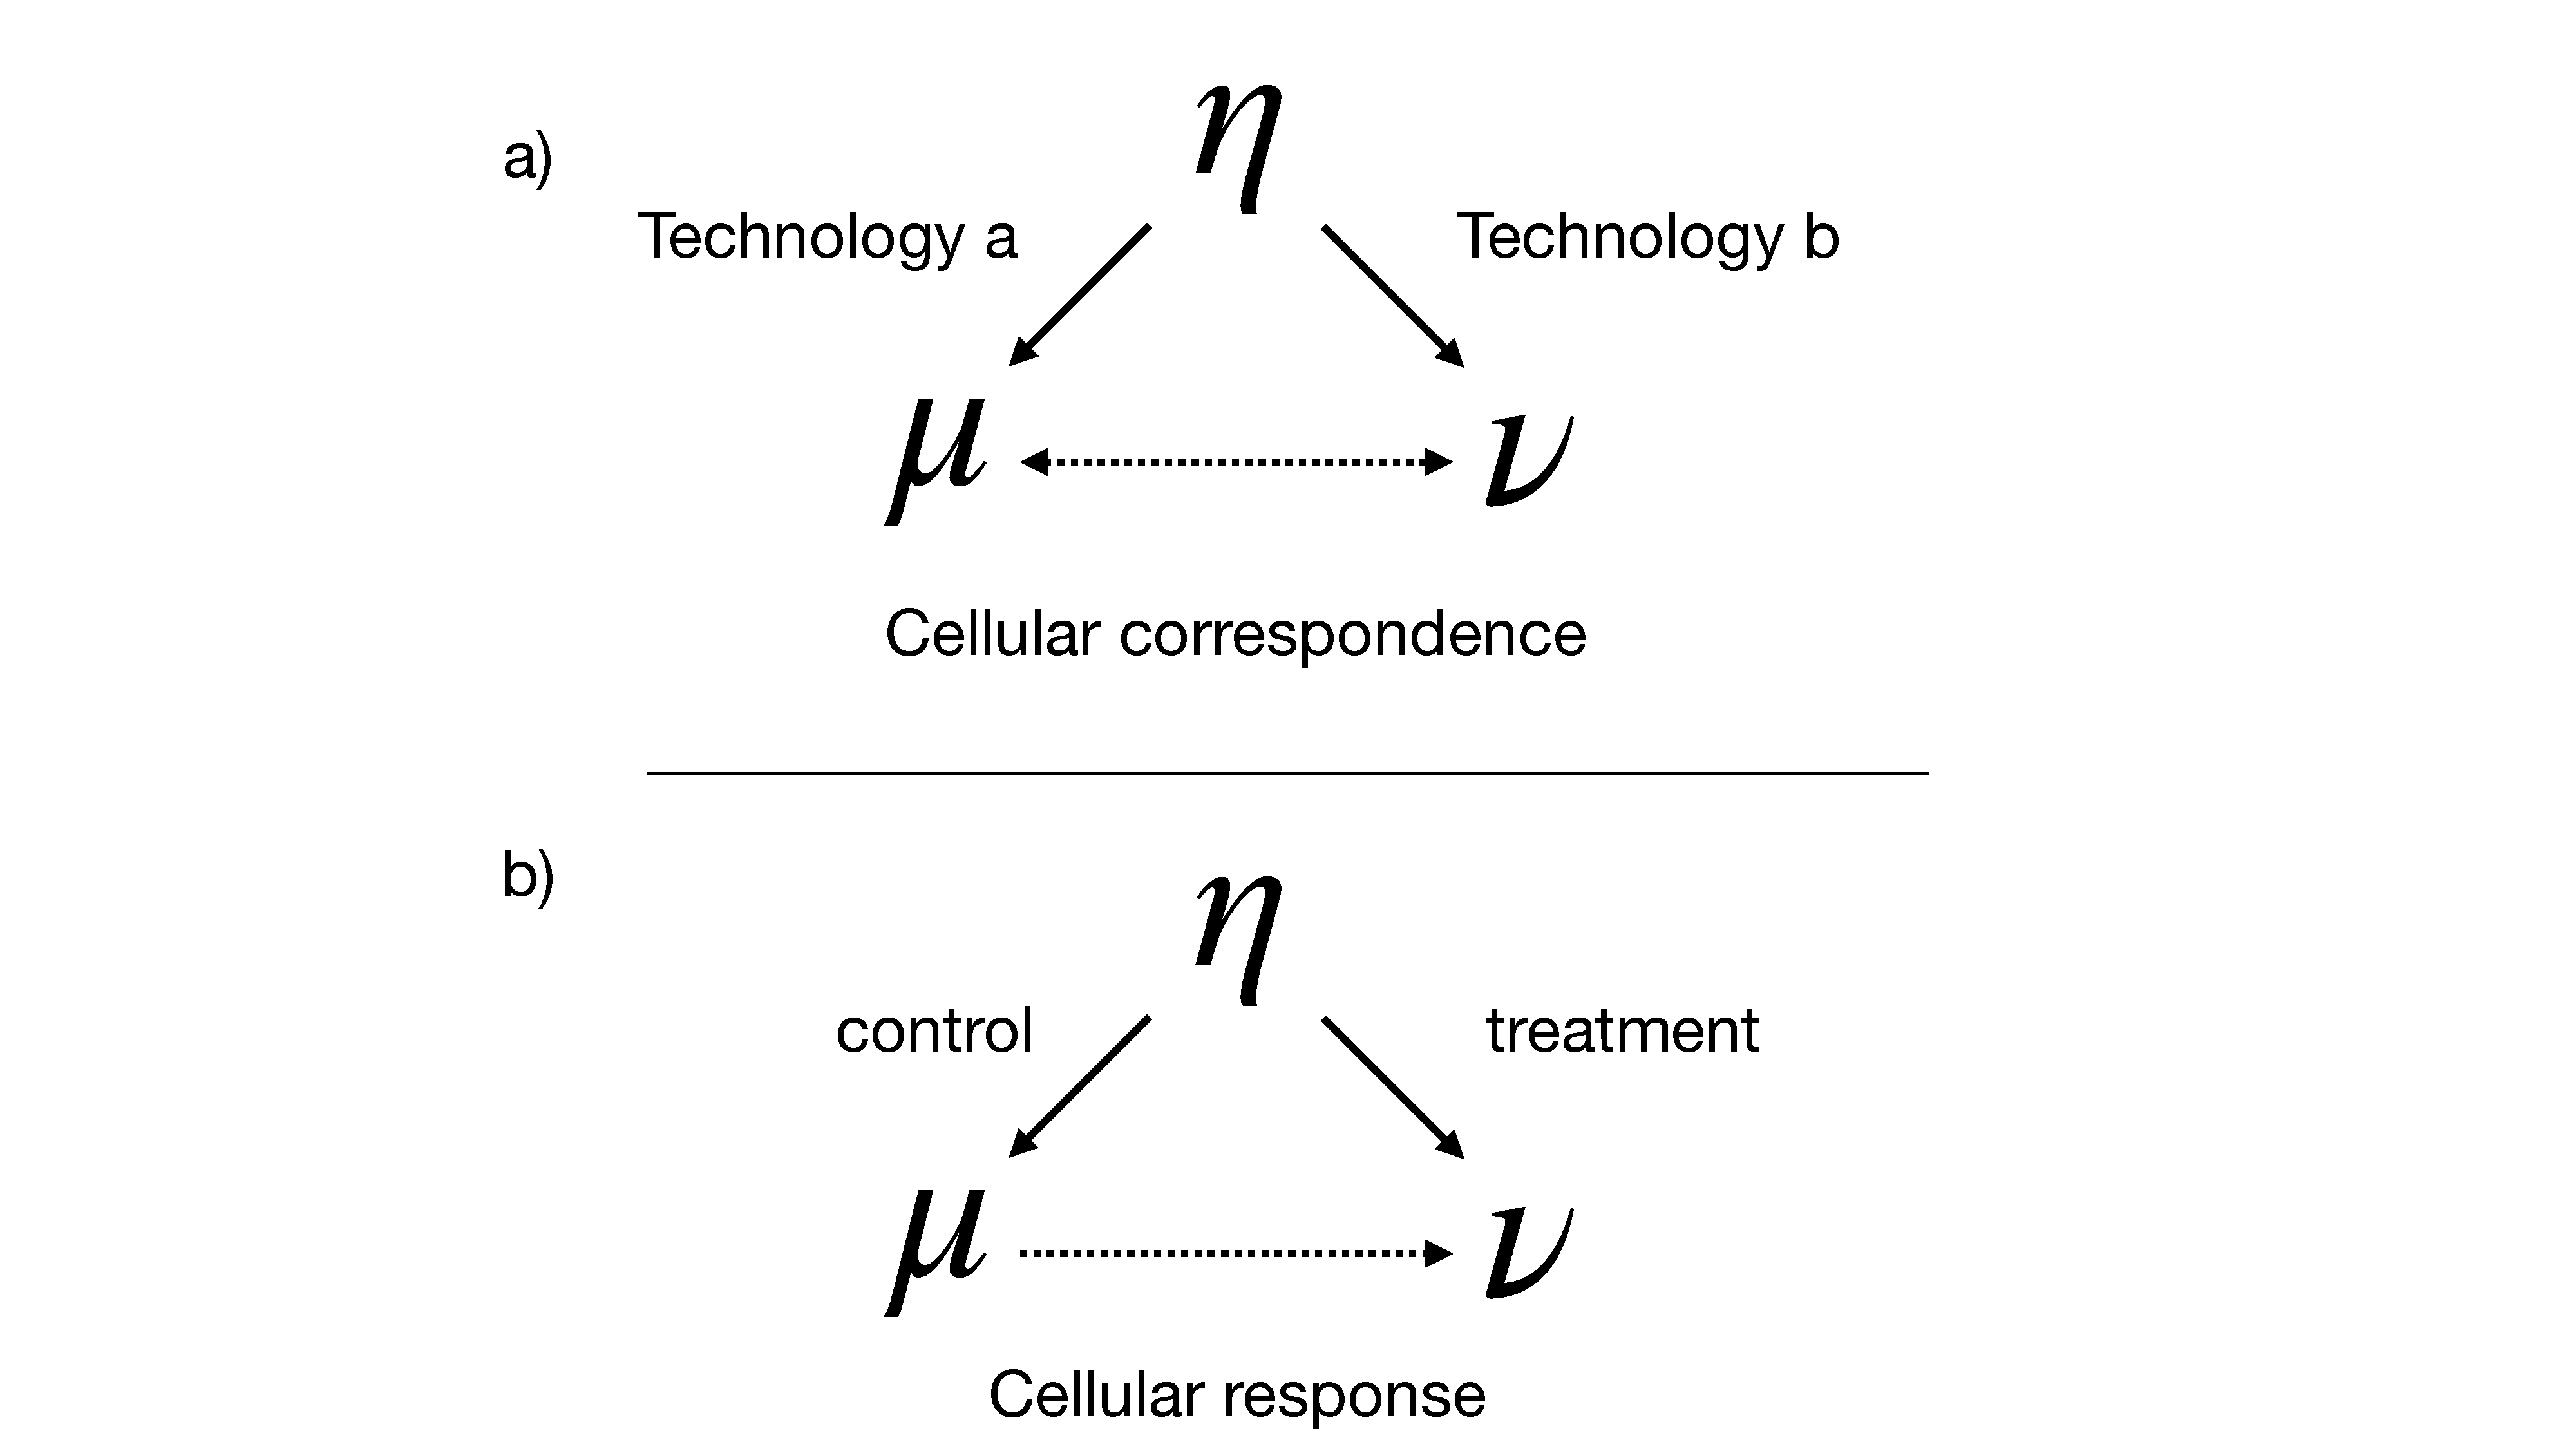
\includegraphics[width=0.95\textwidth]{figures/introduction/thesis-overview-pgm.pdf}
  \end{center}
  \caption{}\label{fig:thesis-overview-pgm}
\end{figure}

\paragraph{Constructing holistic view of cells}
Often it is advantageous to understand cellular state in the context of multiple modalities,
for instance, to understand the joint-wise state of gene expression and protein levels.
Here, $\mu$ and $\nu$ can be considered projects of $\eta$ from some abstract space representing a holistic cellular state into their respective observable domains, e.g. gene expression space or protein space, as summarized in Figure \ref{need}a.
The key complication here is that $\mu$ and $\nu$ are typically in distinct feature spaces that might not have a trivial correspondence.
For instance, the relationship between genes and proteins are known to not be 1-to-1 \cite{edfors2016}.
Chapter \ref{ch:scim} describes SCIM, a framework that performs multi-modal single-cell integration in the absence of corresponding cellular feature sets.

\paragraph{Constructing time-resolved cellular observations}
The cellular responses to perturbations can be considered as a temporal process.
Cells are exposed to some agent of perturbation, such as a drug treatment, that causes a cascade of signal activation within the cell, changing its state.
Here, $\mu$ and $\nu$ can be considered observations of $\eta$ within the same observational domain but under different conditions, summarized in Figure \ref{need}b
Typically $\mu$ will refer to the population treated and profiled with some control condition, while $\nu$ will refer to the population treated with the perturbation of interest and profiled after some time has passed.
The key complication here is that the underlying cellular populations will be heterogeneous in composition and response, and these complicated responses will need to be recovered without access to paired input-output cellular states.
Chapter \ref{ch:cellot} describes CellOT, a framework to learn and predict such heterogenous perturbation responses from uncoupled cellular observations using recent advances in neural optimal transport.
Chapter \ref{ch:cohort} explores the clinical utility of such an approach by applying it to learn and predict the responses of a cohort of melanoma patients to a set of standard-of-care treatments.
